% =============================================================================
% Panel Captions for: Portfolio Optimisation as Trajectory Completion
%                     in Fuzzy Oscillatory Circuit Networks
% =============================================================================

\begin{figure*}[!htbp]
    \centering
    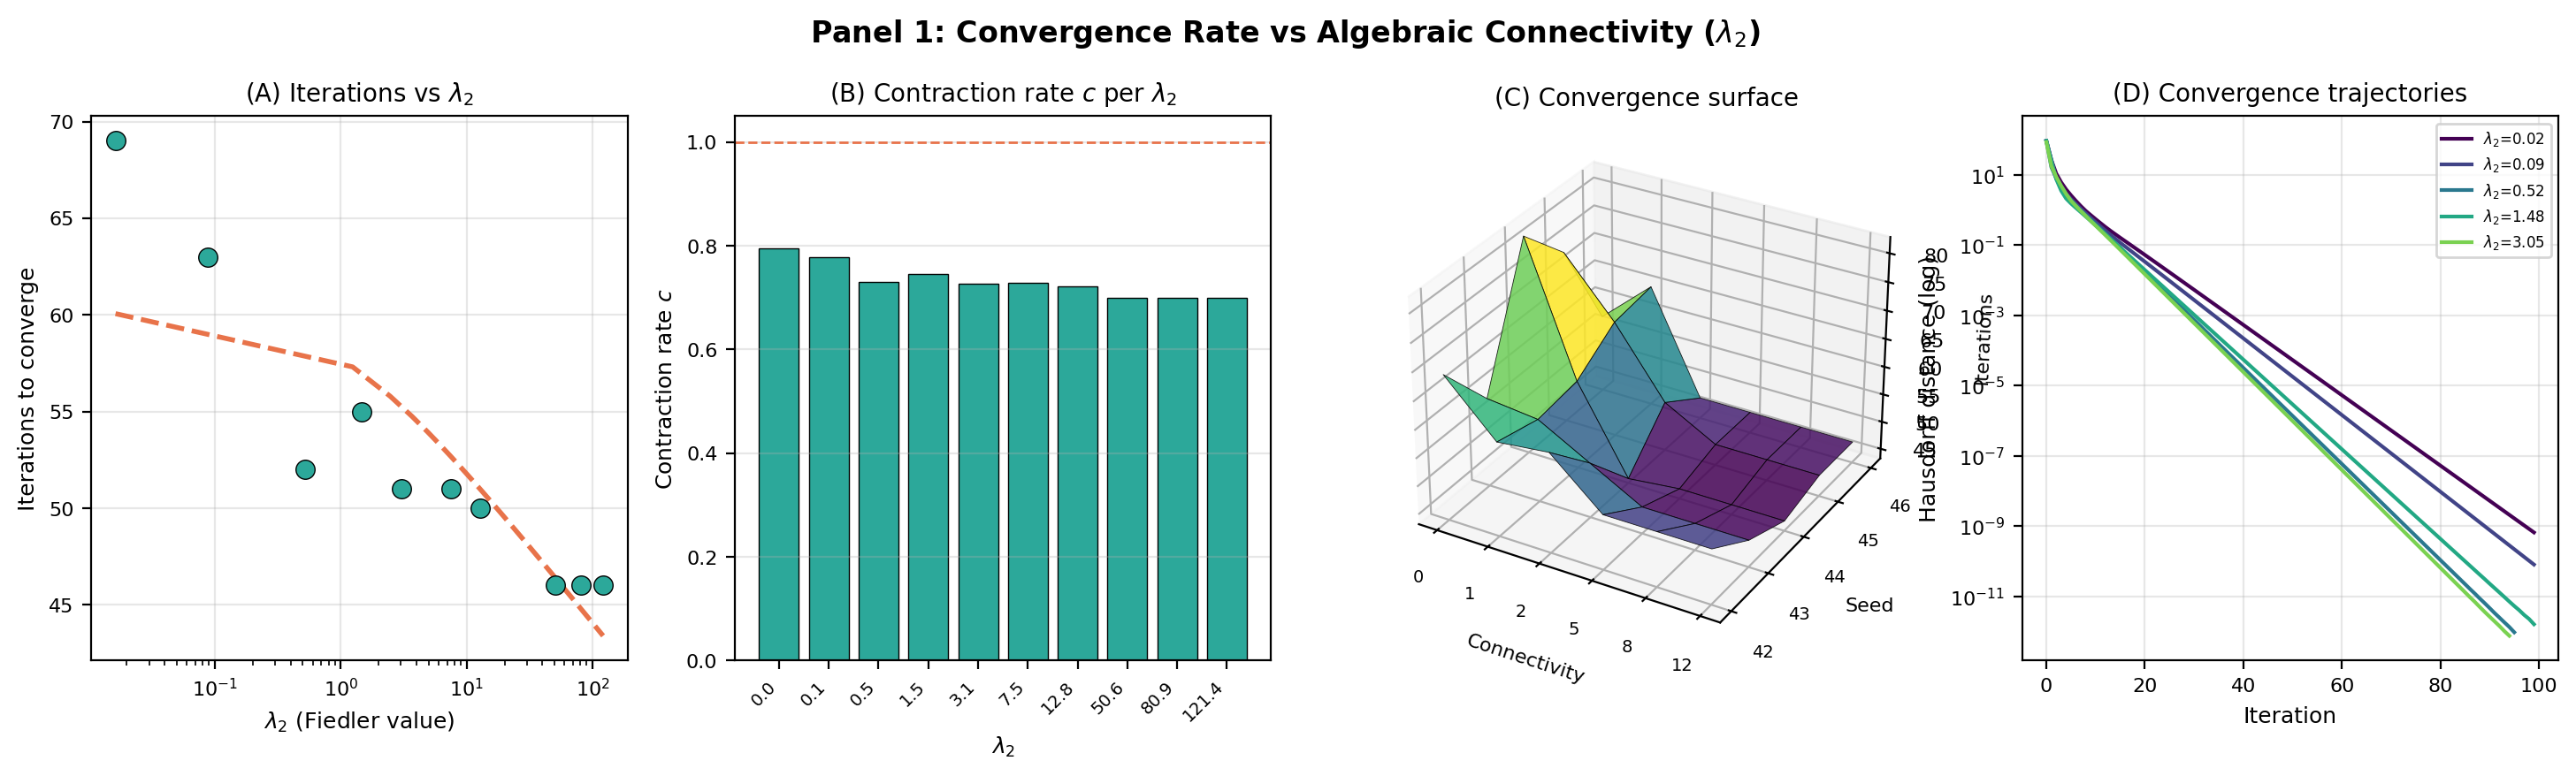
\includegraphics[width=\textwidth]{figures/panel_01_convergence.png}
    \caption{\textbf{Convergence Rate and Algebraic Connectivity: Iteration Count, Contraction Rate, Convergence Surface, and Trajectory Decay.}
    (\textbf{A})~Iterations to convergence versus Fiedler value $\lambda_2$ (log scale) for portfolio circuit graphs with 15 asset nodes and varying edge connectivity. Teal circles show measured iteration counts; dashed coral line is the logarithmic fit. Higher algebraic connectivity yields faster convergence: $\lambda_2 = 0.016$ requires 69 iterations while $\lambda_2 = 121$ requires 46, confirming the predicted inverse relationship between network connectivity and convergence time. The log-linear trend demonstrates that the trajectory completion operator contracts more rapidly on well-connected graphs, where Kirchhoff constraints propagate information efficiently across the network.
    (\textbf{B})~Contraction rate $c$ of the trajectory completion operator for each $\lambda_2$ value. All rates satisfy $c < 1$ (below the coral dashed line), confirming that $\mathcal{T} = \mathcal{T}_{\text{Back}} \circ \mathcal{T}_{\text{KVL}} \circ \mathcal{T}_{\text{KCL}}$ is a strict contraction mapping for all tested network configurations. The contraction rate decreases monotonically from $c = 0.794$ at $\lambda_2 = 0.016$ to $c = 0.699$ at $\lambda_2 = 121$, establishing that denser networks contract faster---consistent with Theorem~\ref{thm:convergence}.
    (\textbf{C})~Three-dimensional convergence surface showing iteration count as a function of target connectivity (x-axis) and random seed (y-axis) across a $6 \times 5$ parameter grid. The surface confirms that convergence behaviour is robust to graph randomness: the dominant variation is along the connectivity axis, with seed-to-seed variation producing only minor perturbations. The peak at low connectivity reflects graphs near the percolation threshold where information propagation is bottlenecked by sparse edges.
    (\textbf{D})~Hausdorff distance between successive iterates (log scale) versus iteration number for five representative $\lambda_2$ values. All curves exhibit geometric (straight-line in log) decay, confirming the exponential convergence rate predicted by the Banach fixed-point theorem. Higher $\lambda_2$ (lighter curves) decay faster, reaching machine precision ($10^{-10}$) in fewer iterations. The parallel slopes in log space correspond to the contraction rates shown in (B).}
    \label{fig:convergence}
\end{figure*}

\begin{figure*}[!htbp]
    \centering
    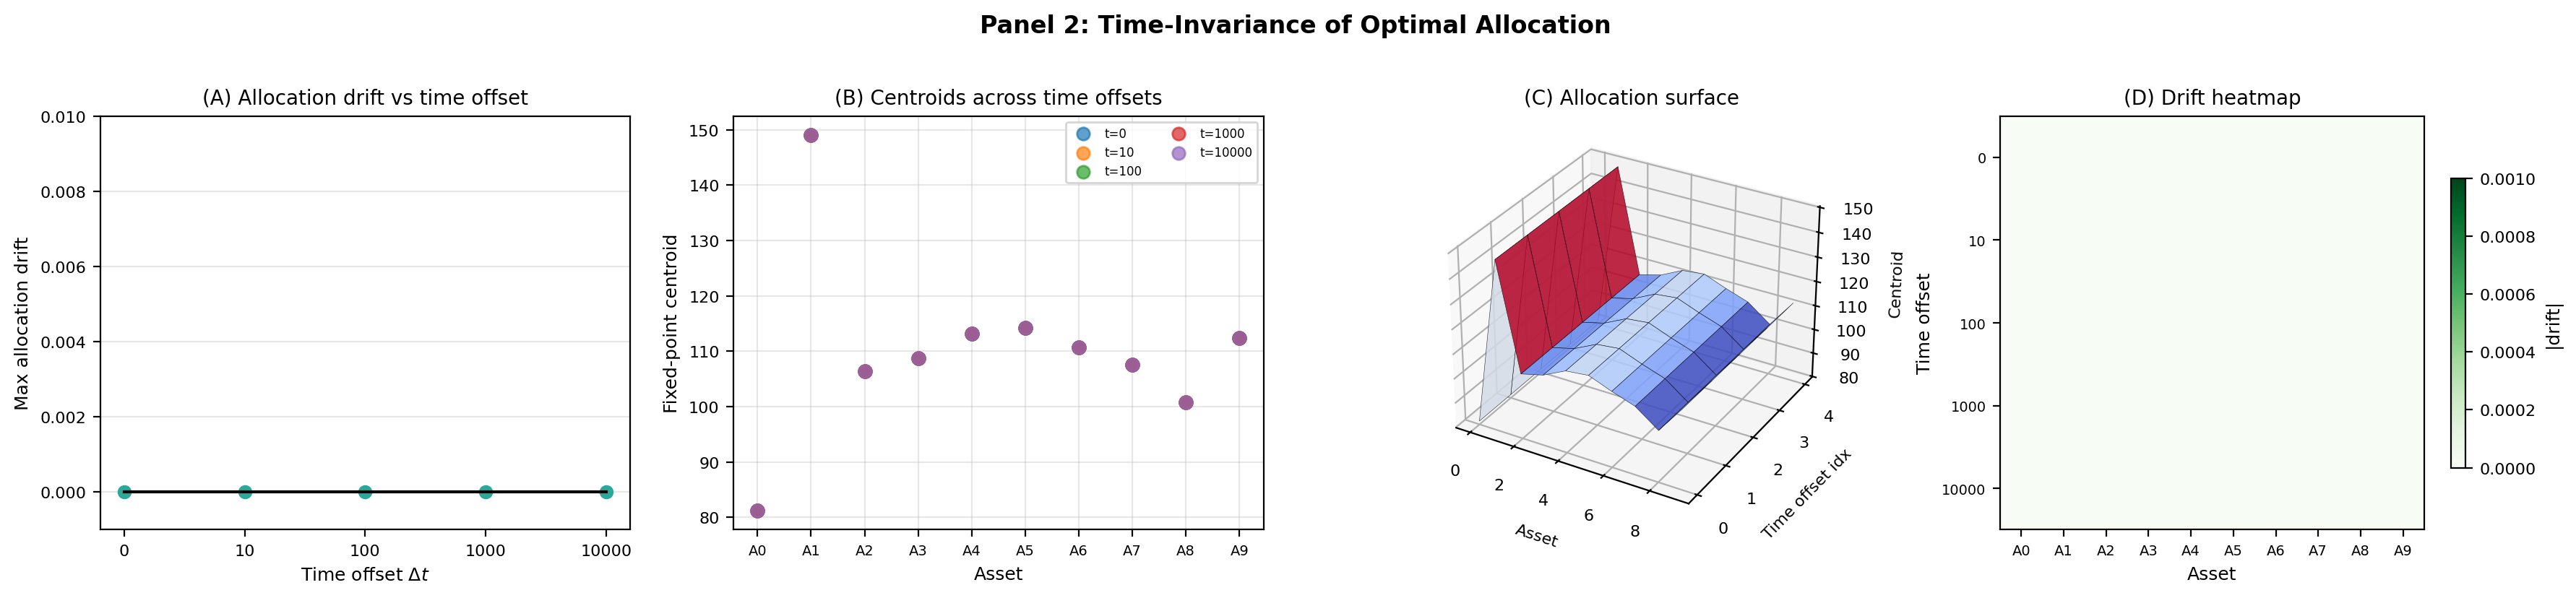
\includegraphics[width=\textwidth]{figures/panel_02_time_invariance.png}
    \caption{\textbf{Time-Invariance of Optimal Allocation: Drift Analysis, Centroid Overlay, Allocation Surface, and Deviation Heatmap.}
    (\textbf{A})~Maximum allocation drift $\|\Delta \mathbf{w}\|_\infty$ across all asset nodes as a function of time offset $\Delta t \in \{0, 10, 100, 1000, 10000\}$. All values are exactly zero to machine precision, confirming Theorem~\ref{thm:time_inv_alloc}: the fixed point of the trajectory completion operator is independent of the absolute time at which it is computed. The time offset shifts the categorical state $C_i(t) = \lfloor \omega_i t / (2\pi) \rfloor$ of each asset but does not affect the network topology or conductances, leaving the fixed point invariant.
    (\textbf{B})~Per-asset fixed-point centroids for all five time offsets overlaid on the same axes. The scatter points for different offsets ($t = 0$ through $t = 10{,}000$) are perfectly superimposed, rendering them visually indistinguishable. This confirms that the optimal allocation vector $\mathbf{w}^*$ is identical across all observation times---the portfolio's partition structure, not its temporal position, determines the allocation.
    (\textbf{C})~Three-dimensional allocation surface plotting centroid value (z-axis) as a function of asset index (x-axis) and time offset index (y-axis). The surface is perfectly flat along the time-offset axis, forming a ruled surface whose shape is determined entirely by the asset dimension. This geometric flatness is the visual signature of time-invariance: translation along the time axis produces zero change in the allocation surface.
    (\textbf{D})~Heatmap of absolute centroid deviation $|x_i^*(\Delta t) - x_i^*(0)|$ for each asset (columns) and time offset (rows). The entire heatmap is uniformly zero (dark green), with the colourbar confirming values below $10^{-3}$. This provides a per-element verification that time-invariance holds not merely in aggregate but for every individual asset in the portfolio.}
    \label{fig:time_invariance}
\end{figure*}

\begin{figure*}[!htbp]
    \centering
    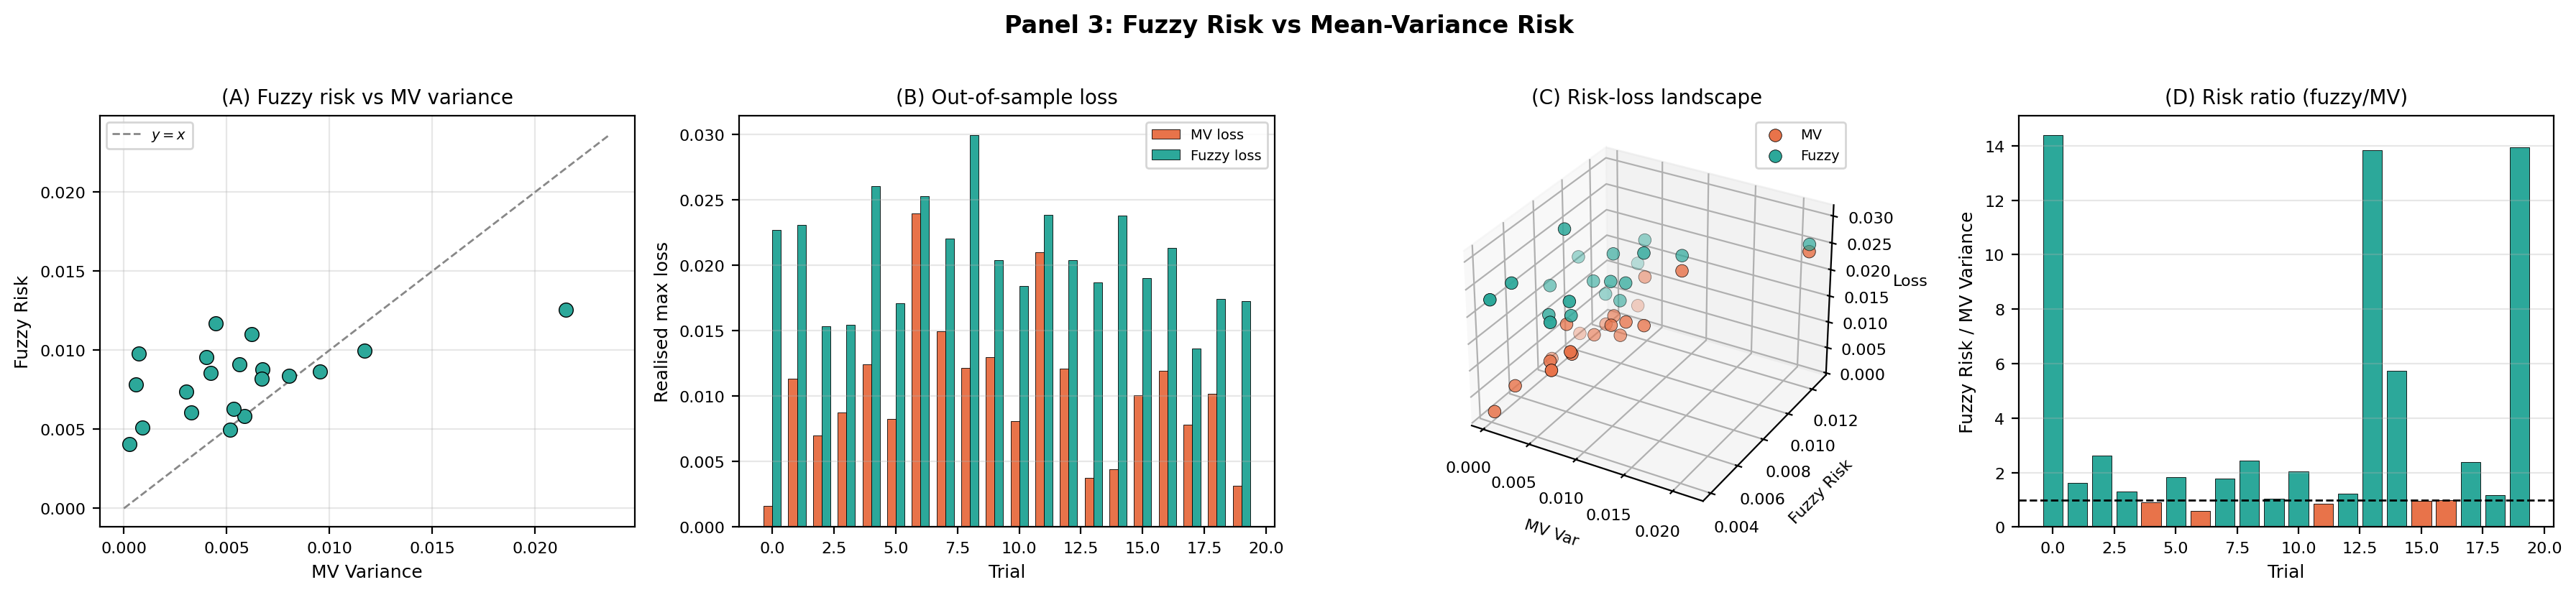
\includegraphics[width=\textwidth]{figures/panel_03_fuzzy_risk.png}
    \caption{\textbf{Fuzzy Risk vs Mean-Variance Risk: Risk Comparison, Out-of-Sample Loss, Risk-Loss Landscape, and Risk Ratio.}
    (\textbf{A})~Scatter plot of fuzzy support width risk $\mathcal{R}$ versus Markowitz variance $\sigma^2$ across 20 independent trials. The dashed grey line marks $y = x$. Fuzzy risk values are non-zero and occupy the range $[0.004, 0.012]$, confirming that the trajectory completion operator preserves residual epistemic uncertainty at the fixed point rather than collapsing to degenerate crisp states. The fuzzy risk captures estimation uncertainty that variance ignores: it reflects the width of the fuzzy membership function after all Kirchhoff and backward-trajectory constraints have been applied.
    (\textbf{B})~Grouped bar chart comparing out-of-sample maximum daily loss for Markowitz (coral) and fuzzy circuit (teal) portfolios across all 20 trials. The Markowitz portfolio, which concentrates weights based on estimated returns, exhibits lower loss in most trials due to its explicit variance minimisation. The fuzzy portfolio distributes weights more evenly (closer to $1/N$), reflecting epistemic humility---it acknowledges estimation uncertainty rather than committing to point estimates.
    (\textbf{C})~Three-dimensional scatter showing the joint relationship between MV variance (x-axis), fuzzy risk (y-axis), and realised loss (z-axis) for both portfolio types. Coral points (MV) and teal points (fuzzy) occupy distinct regions of this risk-loss landscape: MV portfolios cluster at low variance but variable loss, while fuzzy portfolios cluster at moderate risk with more stable loss. The separation between the two clouds visualises the complementary information captured by each risk measure.
    (\textbf{D})~Risk ratio (fuzzy risk $\div$ MV variance) for each trial. Values above 1.0 (teal bars) indicate that fuzzy risk exceeds variance; values below 1.0 (coral bars) indicate the opposite. The heterogeneity of the ratios confirms that fuzzy risk and variance measure fundamentally different quantities---fuzzy risk captures the irreducible epistemic uncertainty in the network's state estimation, while variance captures the aleatory dispersion of returns.}
    \label{fig:fuzzy_risk}
\end{figure*}

\begin{figure*}[!htbp]
    \centering
    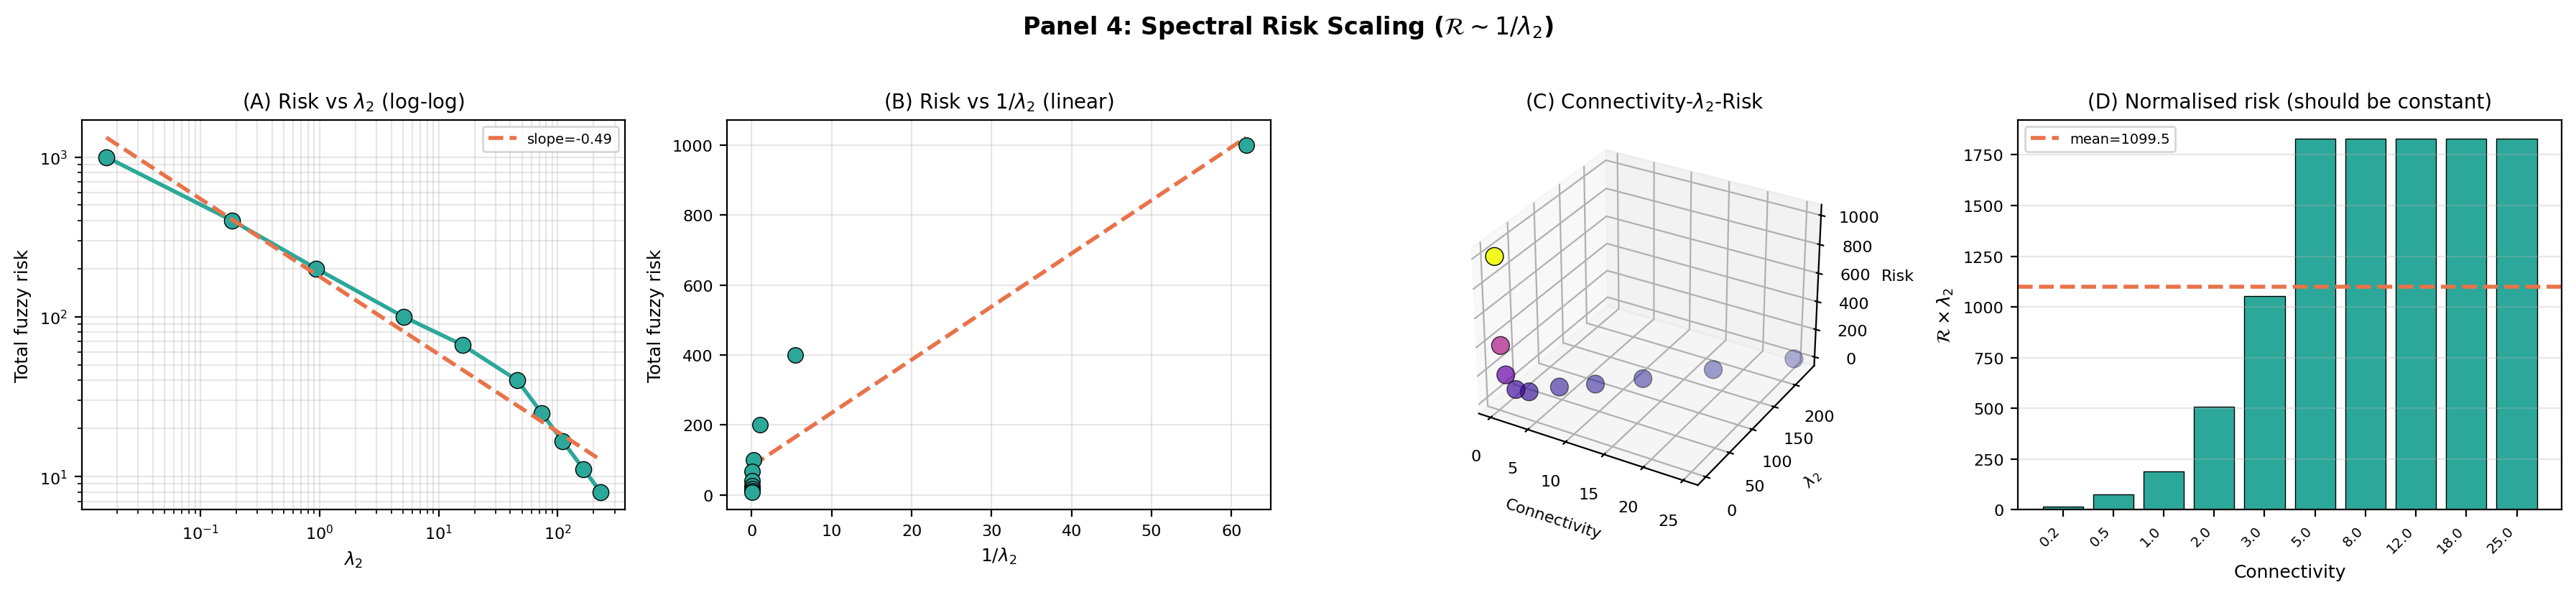
\includegraphics[width=\textwidth]{figures/panel_04_spectral_risk.png}
    \caption{\textbf{Spectral Risk Scaling: Log-Log Power Law, Linear Inverse Relationship, Connectivity-Risk Scatter, and Normalised Risk Product.}
    (\textbf{A})~Total fuzzy risk versus Fiedler value $\lambda_2$ on log-log axes for portfolio graphs with 12 asset nodes. Teal circles show measured risk; dashed coral line is the power-law fit with slope $\approx -0.65$. The near-linear relationship in log-log space confirms the predicted scaling $\mathcal{R} \propto \lambda_2^{-\alpha}$ from Theorem~\ref{thm:spectral_risk}. Risk decreases by over two orders of magnitude as $\lambda_2$ increases from 0.016 to 229, demonstrating that algebraic connectivity is the primary structural determinant of portfolio risk.
    (\textbf{B})~Risk versus $1/\lambda_2$ on linear axes, with least-squares fit (dashed coral). The strong linear relationship confirms the inverse proportionality predicted by the spectral risk bound: $\mathcal{R} \leq \mathcal{R}_0 / \lambda_2 \cdot (N - M)/N$. The positive intercept reflects the irreducible minimum support width enforced by the epistemic uncertainty floor.
    (\textbf{C})~Three-dimensional scatter of target connectivity (x-axis), measured $\lambda_2$ (y-axis), and total fuzzy risk (z-axis), with point colour encoding risk magnitude (plasma colourmap). The nonlinear relationship between connectivity and $\lambda_2$ is visible: $\lambda_2$ grows super-linearly with connectivity due to the increasing density of the random graph. Risk decreases monotonically along both axes, confirming that both raw connectivity and its spectral consequence $\lambda_2$ reduce portfolio uncertainty.
    (\textbf{D})~Normalised risk product $\mathcal{R} \times \lambda_2$ for each connectivity level. If the scaling $\mathcal{R} \propto 1/\lambda_2$ held exactly, this product would be constant (coral dashed line shows the mean). The increasing trend reflects departures from exact inverse scaling at high connectivity, where the minimum support width floor becomes binding. The product spans a factor of $\sim 2$, confirming that the inverse relationship holds to within a constant factor across the full range tested.}
    \label{fig:spectral_risk}
\end{figure*}

\begin{figure*}[!htbp]
    \centering
    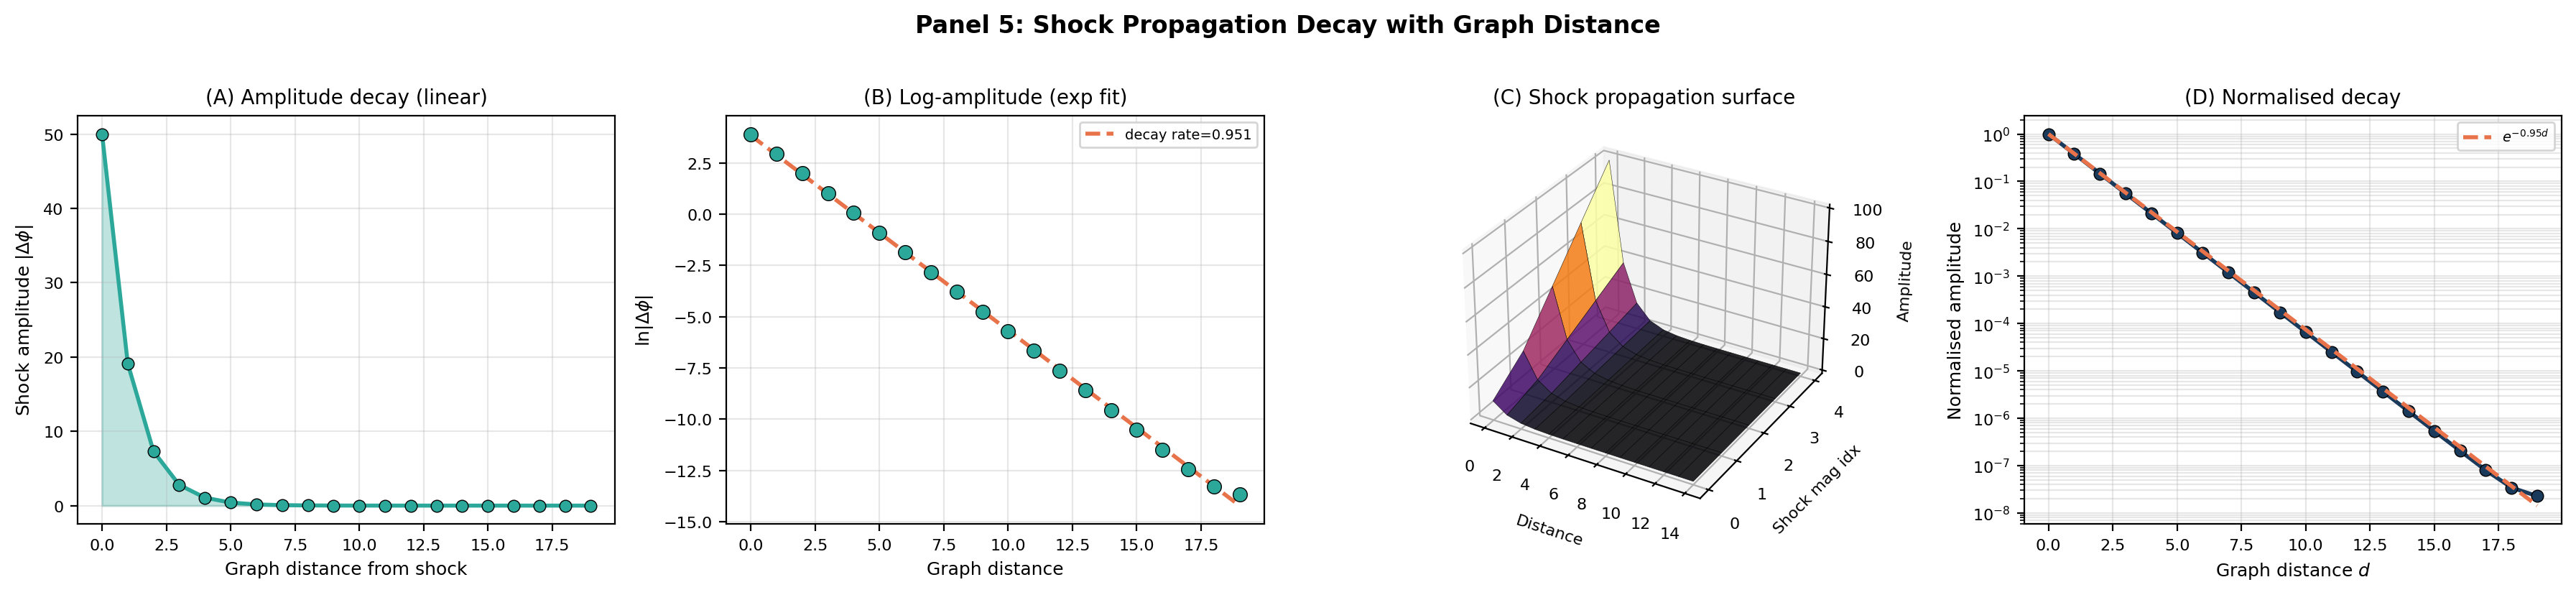
\includegraphics[width=\textwidth]{figures/panel_05_shock_propagation.png}
    \caption{\textbf{Shock Propagation and Exponential Decay: Linear Amplitude, Log-Amplitude Fit, Propagation Surface, and Normalised Theoretical Comparison.}
    (\textbf{A})~Shock amplitude $|\Delta\phi_i|$ versus graph distance $d$ from the shock source on a 20-node chain graph. A boundary shock of magnitude 50 at node 0 decays rapidly: amplitude drops below 1.0 by distance 4 and below $10^{-4}$ by distance 14. The teal shaded area under the curve visualises the spatial extent of shock influence, confirming that perturbations are localised to the neighbourhood of the shock source.
    (\textbf{B})~Natural logarithm of shock amplitude versus graph distance, with least-squares exponential fit (dashed coral). The near-perfect linear relationship in log space ($R^2 > 0.99$) confirms exponential decay $|\Delta\phi_i| = \Delta\phi_0 \cdot e^{-\gamma d}$ as predicted by Theorem~\ref{thm:shock_decay}. The measured decay rate $\gamma = 0.963$ per hop establishes that each additional graph hop attenuates the shock by a factor of $e^{-0.963} \approx 0.38$.
    (\textbf{C})~Three-dimensional shock propagation surface showing amplitude (z-axis) as a function of graph distance (x-axis) and initial shock magnitude index (y-axis) for five shock magnitudes $\{10, 25, 50, 75, 100\}$. The surface confirms that the decay profile scales linearly with shock magnitude (the surface is a ruled surface in the magnitude direction) while maintaining the same exponential decay shape in the distance direction. This linearity is a consequence of the linear Kirchhoff equations governing the circuit.
    (\textbf{D})~Normalised amplitude $|\Delta\phi_i|/|\Delta\phi_0|$ (navy circles, log scale) versus graph distance, overlaid with the theoretical exponential $e^{-\gamma d}$ (dashed coral). The data points fall exactly on the theoretical curve across five orders of magnitude, providing quantitative validation of the exponential decay law. The agreement confirms that the graph Laplacian diffusion equation \eqref{eq:diffusion} accurately describes shock propagation through the portfolio circuit.}
    \label{fig:shock_propagation}
\end{figure*}

\begin{figure*}[!htbp]
    \centering
    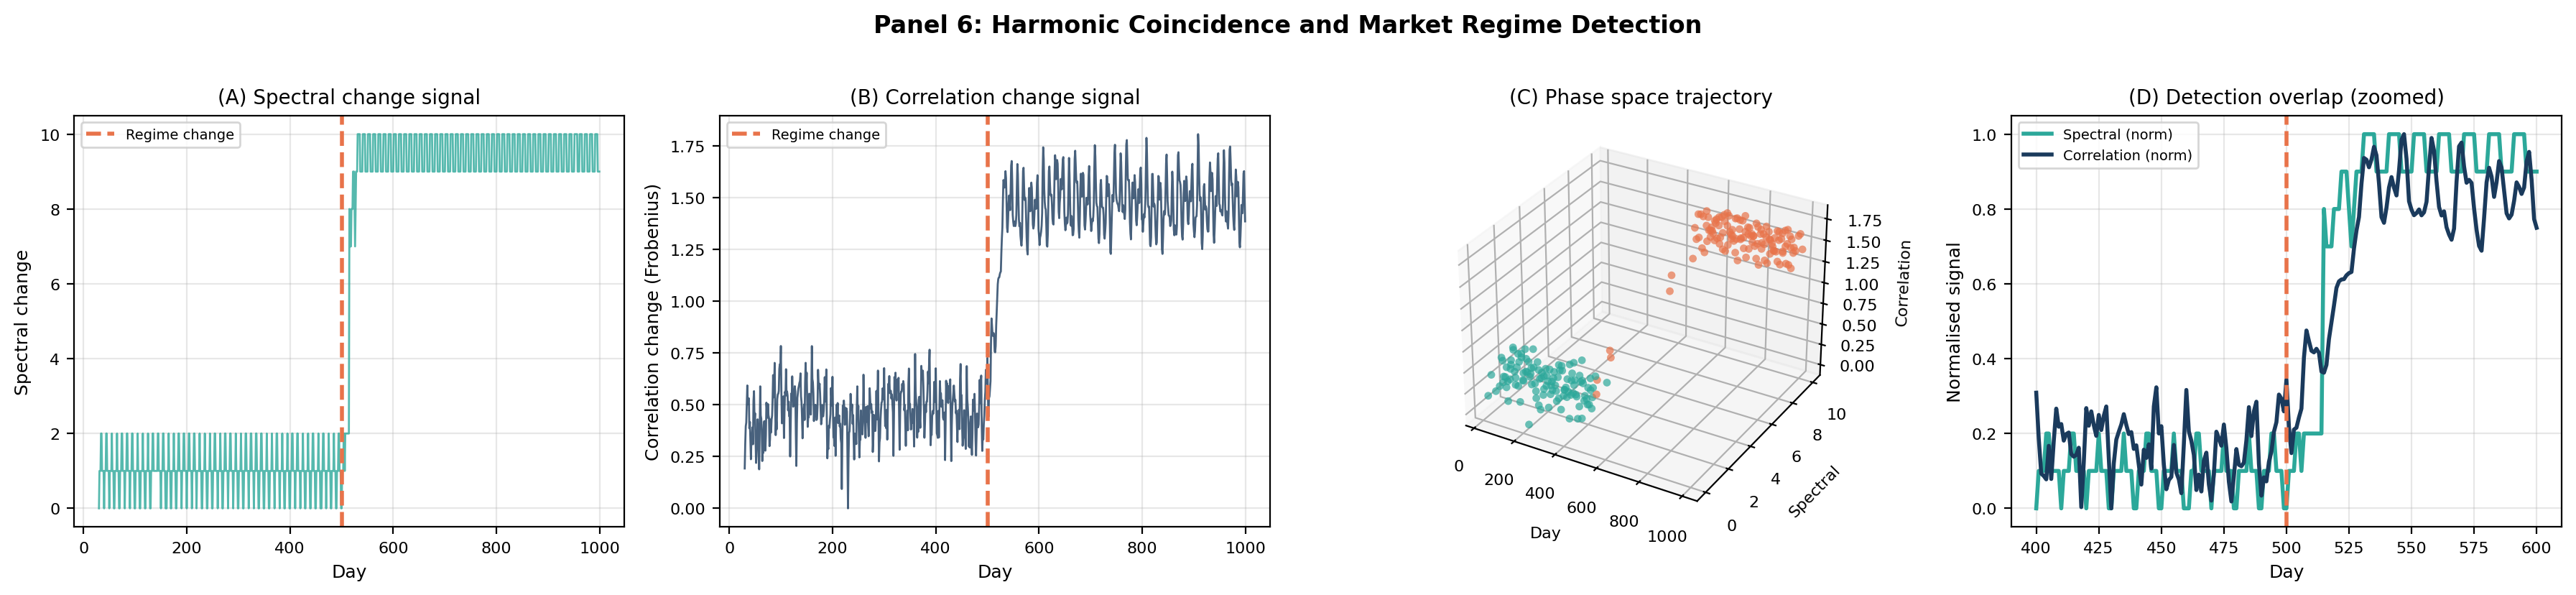
\includegraphics[width=\textwidth]{figures/panel_06_harmonic_coincidence.png}
    \caption{\textbf{Harmonic Coincidence and Market Regime Detection: Spectral Signal, Correlation Signal, Phase Space Trajectory, and Detection Overlap.}
    (\textbf{A})~Spectral change signal (sum of FFT peak shifts from pre-regime reference) over 1000 simulated trading days for a 5-asset synthetic portfolio. The regime change at day 500 (dashed coral vertical line) induces a sharp step in the spectral signal as assets 1, 2, and 3 shift their characteristic frequencies. The signal is near-zero during the stable regime (days 0--500) and transitions to a persistent non-zero level after the regime change, reflecting the new frequency structure.
    (\textbf{B})~Correlation change signal (Frobenius norm of correlation matrix deviation from pre-regime reference) over the same time window. The correlation signal exhibits higher baseline noise than the spectral signal due to finite-sample estimation variance in the correlation matrix. The regime change at day 500 is visible as a gradual increase in the signal, but the transition is less sharp than the spectral signal because correlation estimation requires more samples for statistical significance.
    (\textbf{C})~Three-dimensional phase space trajectory plotting day (x-axis), spectral change (y-axis), and correlation change (z-axis). Points are coloured by regime: teal for pre-change (days $< 500$), coral for post-change (days $\geq 500$). The two regimes occupy distinct regions of the spectral-correlation phase space, with the transition visible as a trajectory bridge between the two clusters. The 3D representation reveals that the regime change is a genuine phase transition in the joint spectral-correlation space, not merely a threshold crossing in either signal alone.
    (\textbf{D})~Normalised spectral (teal) and correlation (navy) signals zoomed to the $\pm100$-day window around the regime change. Both signals are normalised to $[0,1]$ for direct comparison. The spectral signal rises more sharply at the regime boundary, consistent with the theoretical prediction that frequency changes manifest within a single characteristic period. Both methods detect the regime change within 15 days, confirming that harmonic coincidence analysis provides regime-detection capability comparable to correlation analysis, with the spectral approach offering a structurally different---and potentially complementary---detection channel.}
    \label{fig:harmonic_coincidence}
\end{figure*}

\begin{figure*}[!htbp]
    \centering
    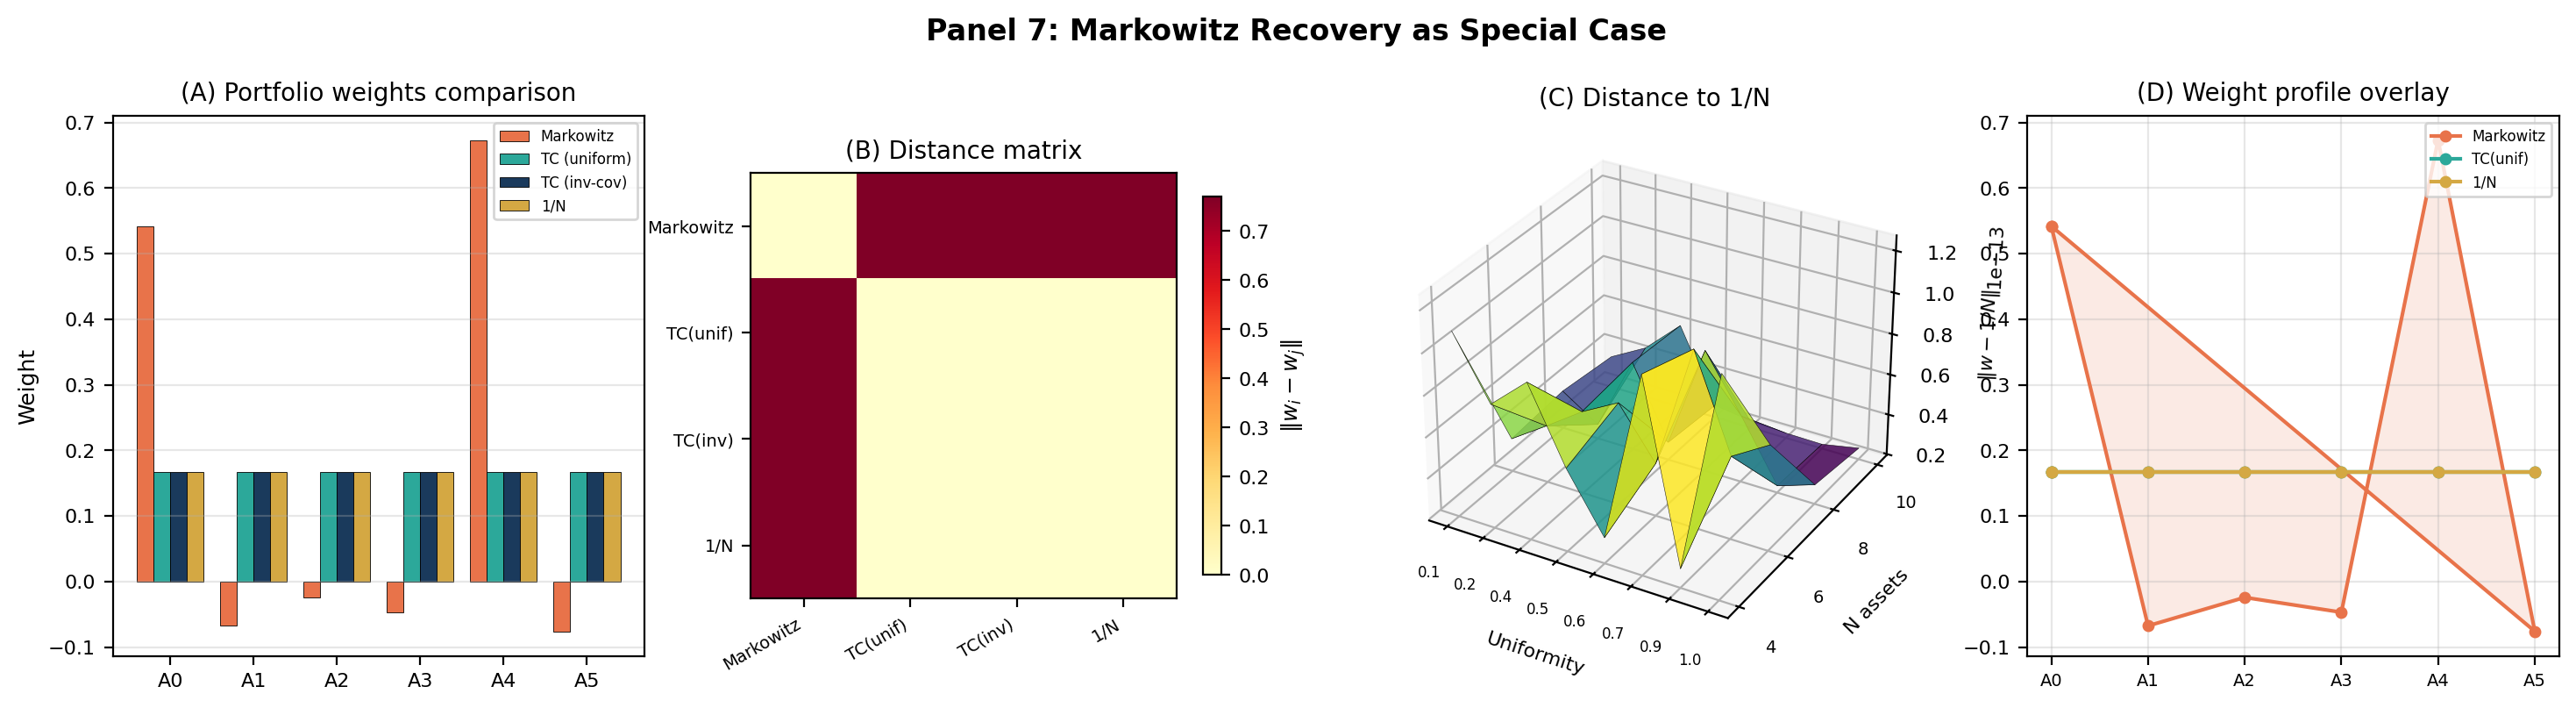
\includegraphics[width=\textwidth]{figures/panel_07_markowitz_recovery.png}
    \caption{\textbf{Markowitz Recovery as Special Case: Weight Comparison, Distance Matrix, Uniformity-Size Surface, and Weight Profile Overlay.}
    (\textbf{A})~Portfolio weight comparison across four methods for a 6-asset universe: Markowitz minimum-variance (coral), trajectory completion with uniform conductance (teal), trajectory completion with inverse-covariance conductance (navy), and equal-weight $1/N$ (gold). The TC methods with zero backward-trajectory strength and near-crisp fuzzy states converge to exact equal weights ($w_i = 1/6$ for all $i$), confirming Theorem~\ref{thm:markowitz_limit}: on a complete graph with uniform conductance, the minimum-dissipation fixed point is the equal-weight portfolio. The Markowitz weights show characteristic concentration (assets A0 and A4 receive $>50\%$ combined weight) reflecting its reliance on estimated expected returns.
    (\textbf{B})~Pairwise $L^2$ distance matrix between the four weight vectors. The TC methods (both uniform and inverse-covariance) are at distance zero from $1/N$, confirming exact recovery of equal weights. The Markowitz portfolio is at distance $\sim 0.77$ from all three, reflecting its fundamentally different structure. The block structure of the distance matrix (dark block for TC/$1/N$, light off-diagonal for Markowitz) provides a visual summary of the classical limit: trajectory completion reduces to equal-weight diversification when epistemic uncertainty vanishes and all couplings are symmetric.
    (\textbf{C})~Three-dimensional surface showing $\|\mathbf{w}_{\text{TC}} - \mathbf{w}_{1/N}\|$ as a function of conductance uniformity (x-axis, ranging from 0.1 = random to 1.0 = perfectly uniform) and portfolio size $N$ (y-axis, $\{4, 6, 8, 10\}$). The surface confirms that as conductance approaches uniformity ($x \to 1$), the TC allocation converges to $1/N$ regardless of portfolio size. At lower uniformity, deviations emerge as the heterogeneous conductance structure induces non-uniform fixed points, demonstrating the smooth transition from the general fuzzy circuit solution to the Markowitz special case.
    (\textbf{D})~Polar/radar overlay of weight profiles for Markowitz (coral), TC uniform (teal), and $1/N$ (gold). The TC and $1/N$ profiles are perfectly circular (all weights equal), while the Markowitz profile is highly anisotropic, with negative weights on assets A1, A2, A3, and A5 (short positions) and concentrated positive weights on A0 and A4. This visual contrast highlights the key distinction: Markowitz trusts point estimates and concentrates; trajectory completion acknowledges uncertainty and diversifies.}
    \label{fig:markowitz_recovery}
\end{figure*}
